\chapter{Test}
\label{chap:test}

The application is futile without a connection to the backend. This is what allows the user to login and afterwards receive data for the user to look at and work with. It is crucial for the application that the data can be retrieved and that the data corresponds to the executed HTTP request and is returned in the correct format. Additionally, the developer working with the API should be able to identify what happened to a failed HTTP request. Based on these arguments, we decided to perform functional testing on our backend, from the perspective of a developer using the API. 

In effect we performed a variation of functional testing - since we are not working with a customer we cannot perform testing based on customer specifications or customer design-documents. Instead we test for correct functionality in a sub-part of the whole system. In one case it means accessing an exposed web service with a HTTP request, which will cause the backend to retrieve data from the database, serialize it to JSON and return it to the client. In another case this means accessing an exposed web service HTTP request that will receive a JSON formatted object, store it in the database and return whether it was stored successfully or not.

To perform the functional testing we use a tool called \textit{Fiddler Web Debugger}. It is a free web debugging proxy for any browser, system or platform\cite{fiddler}. Fiddler provides a feature to compose HTTP requests, and a GUI to look at the status of the requests as well as the response message. 

Once we determine what we want to test, we structure the test in three simple steps as follows.
\begin{itemize}
\item Create input data
\item Determine output data
\item Compare the result with the desired output data
\end{itemize}

This test was performed on all 46 web service HTTP requests exposed through our RESTful API. For the report, a single of these tests is used for explanation. and description of how it was tested. An example of unexpected errors is also included. The test example is for the \texttt{AddAccount} POST-request which should return one of five outputs. These are as follows.

\subsection{AddAccount}
\begin{figure}
\centering
\includegraphics[width=0.95\textwidth]{Pictures/test/composeraddaccount.png}
\caption{AddAccount}
\label{fig:composeraddaccount}
\end{figure}

\begin{figure}
	\centering
	% 1
	\begin{subfigure}[b]{\textwidth}
		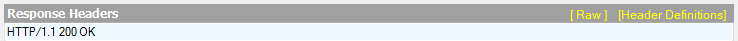
\includegraphics[width=\textwidth]{Pictures/test/AddAccountOK.png}
		\caption{OK}
		\label{fig:AddAccountOK}
	\end{subfigure}
	% 2
	\begin{subfigure}[b]{\textwidth}
		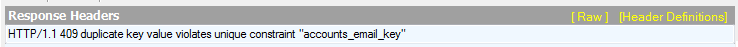
\includegraphics[width=\textwidth]{Pictures/test/AddAccountduplicate.png}
		\caption{Duplicate Key}
		\label{fig:AddAccountduplicate}
	\end{subfigure}
	% 3
	\begin{subfigure}[b]{\textwidth}
		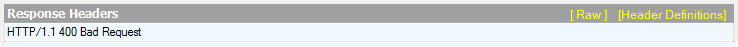
\includegraphics[width=\textwidth]{Pictures/test/AddAccountbadrequest.png}
		\caption{Bad Request}
		\label{fig:AddAccountbadrequest}
	\end{subfigure}
	% 4
	\begin{subfigure}[b]{\textwidth}
		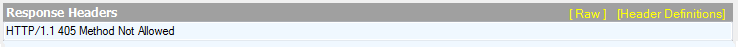
\includegraphics[width=\textwidth]{Pictures/test/AddAccountmethodnotallowed.png}
		\caption{Method Not Allowed}
		\label{fig:AddAccountmethodnotallowed}
	\end{subfigure}
	% 5
	\begin{subfigure}[b]{\textwidth}
		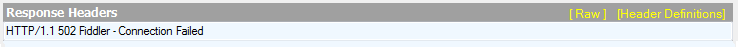
\includegraphics[width=\textwidth]{Pictures/test/AddAccountconnectionfailed.png}
		\caption{Connection Failed}
		\label{fig:AddAccountconnectionfailed}
	\end{subfigure}
	\caption{Results gathered from testing AddAccount}
	\label{fig:addaccountresults}
\end{figure}

\paragraph{OK}
In this case, the desired functionality is for the backend to insert a new row in the database-table called accounts, with the content specified in JSON-format listed in the composer figure \ref{fig:composeraddaccount}. 

For the given response message, see figure \ref{fig:AddAccountOK}, which is indeed the desired result and the test-case succeeded.
\paragraph{Duplicate Key}
In this case, the desired functionality is for the backend to detect that there already exists a row in the database with the same data as the one entered in the composer figure \ref{fig:composeraddaccount}. This will for an account only be possible for attributes marked with the UNIQUE identifier. In this case, it can only be the \texttt{email}, because the \texttt{accountid} is assigned by the database itself. This error was generated by executing the exact same HTTP request which has just returned an HTTP header with the OK result.

For the database violations, multiple types of database error-messages can occur, allowing for easy detection of the error made by the developer.

For the given response-message, see figure \ref{fig:AddAccountduplicate}, this is indeed the desired result and the test-case succeeded.
\paragraph{Bad Request}
In this case, the desired functionality is for the backend to tell the developer that they entered a bad request. This error can be generated in two ways. The first can be generated by corrupting the JSON formatting. This mean the standard for JSON-formatting was violated, which the backend should detect. The second error can be generated by changing the application/json in the composer figure \ref{fig:composeraddaccount} to application/xml. This means that the request body must be formatted as xml, which it obviously is not, hereby the error.

For the given response-message, see figure \ref{fig:AddAccountbadrequest}, this is indeed the desired result and the test-case succeeded.
\paragraph{Method Not Allowed}
The Web Service defined the type of \texttt{AddAccount} to be POST. Defining the HTTP requests to be any other type will result in the Method Not Allowed error. This error can be generated by changing the method-type to any other type than POST.

For the given response-message, see figure \ref{fig:AddAccountmethodnotallowed}, this is indeed the desired result and the test-case succeeded.
\paragraph{Connection Failed}
We turned the API off and executed an HTTP request trying to access the API. This should result in the connection failed error. 

For the given response-message, see figure \ref{fig:AddAccountconnectionfailed}, this is indeed the desired result and the test-case succeeded.

\subsection{GetRecipeById}
A few cases did not initially provide the expected results. The most interesting case of this happening was with the method called \texttt{GetRecipeById}.
This request returns a targeted recipe from the database, given that the provided ID exists in the database. During the early stages of the web service implementation, we had a strange error occur on the client side (running Java). The program kept throwing an exception: \texttt{java.net.SocketException: ECONNRESET (Connection reset by peer)}\cite{socketexception}. The exception basically says that the connection was terminated by the host, without returning an answer. This was strange because the web service was supposed to return a recipe if the ID existed or respond with HTTP status code 204 (No Content), if it did not exist. The error occurred because the web service did not properly get told by the \texttt{DBController} that it did not find a recipe with the provided id, and when the web service stood without a recipe to return, as well as no confirmation that no such recipe existed, it just terminated the connection to the client. We fixed the error by altering the way the \texttt{DBController} handles empty queries, and as a result, it will now properly inform the client with 204 No Content.


